\chapter{Rezultate experimentale}
\label{cap:rezultate}

În cadrul acestui capitol vor fi prezentate o serie de rezultate prin care poate fi analizată eficiența metodei propuse în cadrul capitolui\ref{cap:contributii}.

\section{Analiza strategiilor de selecție a lanțurilor de tipare închise}

Pentru rezultate prezentate în cadrul următoarelor tabele s-au folosit jumătate dintre cuvintele silabisite din setul de date RoSyllabiDict ($\sim200.000$) pentru identficarea de tipare frecvente. 

Pentru validarea strategiilor s-au extras aleatoriu, 10.000 de cuvinte din a doua jumătate a setului de cuvinte RoSyllabiDict.

În cazul strategiei care selectează silabisirea idenficată cu cele mai multe lanțuri de tipare închise, rezultate sunt ilustrate în cadrul tabelei ~\ref{table:counting}.

\begin{table}[h!]
\centering
\begin{tabular}{|c|c|c|c|c|}
\hline
suport minim & $m_d$ & $\sum m_w$ & $\%{m_w}$ & cuvinte nedespărțite\\ 
\hline
\hline
50 & 0.898810282887619 & 4719 & 51.85 & 899\\ 
\hline
45 & 0.895689133288429 & 4644 & 50.53 & 810\\ 
\hline
40 & 0.893229396558503 & 4665 & 50.28 & 722\\ 
\hline
35 & 0.89376043637831 & 4740 & 50.68 & 648\\ 
\hline
30 & 0.890320159357963 & 4681 & 49.55 & 553\\ 
\hline
25 & 0.889120134369591 & 4713 & 49.4 & 459\\ 
\hline
20 & 0.888821085026373 & 4808 & 49.85 & 355\\ 
\hline
15 & 0.886419928605455 & 4773 & 49 & 260\\ 
\hline
10 & 0.875989677334146 & 4210 & 42.84 & 173\\ 
\hline
5 & 0.859792028980429 & 3672 & 37.01 & 78\\ 
\hline\end{tabular}
\caption{Evaluarea strategiei bazată pe numărul de lanțuri de tipare închise echivalente} 
\label{table:counting}
\end{table}

În cadrul tabelei ~\ref{table:overlapping} sunt ilustrate rezultate analizei în cazul strategiei bazată pe suprapuneri. 

\begin{table}[h!]
\centering
\begin{tabular}{|c|c|c|c|c|}
\hline
suport minim & $m_d$ & $\sum m_w$ & $\%{m_w}$ & cuvinte nedespărțite\\ 
\hline
\hline
50 & 0.934182795192563 & 5669 & 62.29 & 899\\ 
\hline
45 & 0.933385818781609 & 5698 & 62 & 810\\ 
\hline
40 & 0.935090134710169 & 5830 & 62.84 & 722\\ 
\hline
35 & 0.935032634560768 & 5908 & 63.17 & 648\\ 
\hline
30 & 0.934206185385081 & 5933 & 62.8 & 553\\ 
\hline
25 & 0.935714036164661 & 6036 & 63.26 & 459\\ 
\hline
20 & 0.934152429276784 & 6076 & 63 & 355\\ 
\hline
15 & 0.936083160365696 & 6211 & 63.77 & 260\\ 
\hline
10 & 0.936303244543237 & 6269 & 63.79 & 173\\ 
\hline
5 & 0.928531534060846 & 5916 & 59.63 & 78\\ 
\hline\end{tabular}
\caption{Evaluarea strategiei bazate pe nivelul de suprapunere} 
\label{table:overlapping}
\end{table}

Iar în cadrul tabelei ~\ref{table:shortest} este ilustrată evaluarea strategiei bazate pe lungimea lanțurilor de tipare închise.

\begin{table}[h!]
\centering
\begin{tabular}{|c|c|c|c|c|}
\hline
suport minim & $m_d$ & $\sum m_w$ & $\%{m_w}$ & cuvinte nedespărțite\\  
\hline
\hline
50 & 0.948261855927185 & 6392 & 70.23 & 899\\ 
\hline
45 & 0.947471781784847 & 6458 & 70.27 & 810\\ 
\hline
40 & 0.948916493018081 & 6588 & 71.01 & 722\\ 
\hline
35 & 0.950700978994344 & 6727 & 71.93 & 648\\ 
\hline
30 & 0.950471973129913 & 6820 & 72.19 & 553\\ 
\hline
25 & 0.952801443394629 & 6985 & 73.21 & 459\\ 
\hline
20 & 0.954658800101994 & 7171 & 74.35 & 355\\ 
\hline
15 & 0.956975673054947 & 7337 & 75.33 & 260\\ 
\hline
10 & 0.959539699499725 & 7500 & 76.32 & 173\\ 
\hline
5 & 0.958024515826585 & 7633 & 76.93 & 78\\ 
\hline\end{tabular}
\caption{Evaluarea strategiei bazate pe lungimea lanțurilor de tipare închise} 
\label{table:shortest}
\end{table}

La nivel comparativ, în cadrul figurilor ~\ref{fig:strategies-word} și \ref{fig:strategies-point} se poate observa evoluția preciziei la nivelul ambelor metrici definite anterior. 


\begin{figure}[h!]
    \centering
    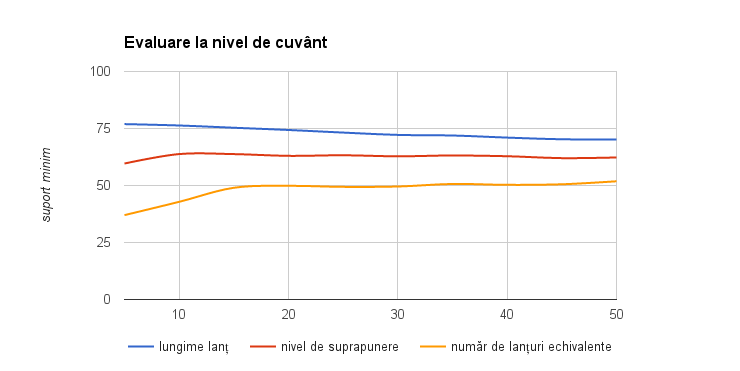
\includegraphics[width=1\textwidth]{figures/strategies-word.png}
    \caption{Evaluare comparativă a strategiilor ($\%m_w$)}
    \label{fig:strategies-word}
\end{figure}


\begin{figure}[h!]
    \centering
    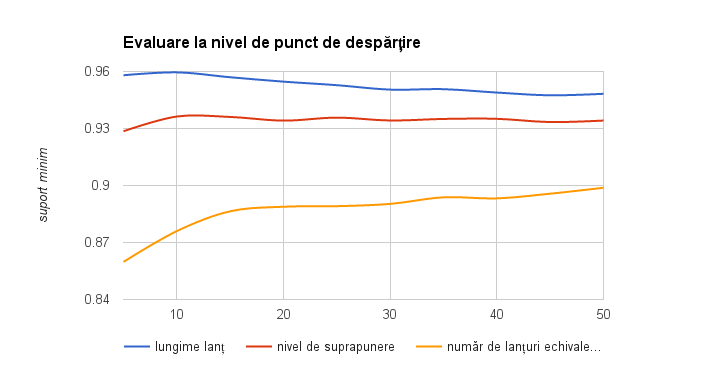
\includegraphics[width=1\textwidth]{figures/strategies-point.png}
    \caption{Evaluare comparativă a strategiilor ($m_d$)}
    \label{fig:strategies-point}
\end{figure}

Din cele două figuri putem trage două concluzii:

\begin{itemize}
\item strategia bazată pe lungimea lanțului de tipare închis performează cel mai bine. 
\item cele două metrici reflectă aleași rezultate. 
\end{itemize}

\newpage
\section{Analiza comparativă cu alte metode de silabisire}

Pentru a încadra rezultatele relativ la alte abordări, au fost preluate rezultate din cadrul articolului ~\cite{bib:dinu2013romanian} și sunt prezentate în cadrul tabelei ~\ref{table:comparison}. 

Trebuie menționat că deși metoda prezentată în cadrul acestei lucrări, nu excelează la precizie, aceasta prezintă un nivel ridicat de genericitate. în cadrul tabelului 

\begin{table}[h!]
\centering
\begin{tabular}{|c|c|c|c|c|}
\hline
Abordare & Acuratețe la nivel de cuvânt\\  
\hline
\hline
RULE & 60,67\%\\ 
\hline
 \textbf{metoda prezentată în cadrul acestei lucrări} & \textbf{76,93\%} \\ 
\hline
SVM & 90,46\%\\ 
\hline
CRF & 95,25\%\\ 
\hline\end{tabular}
\caption{Evaluare comparativă cu alte soluții} 
\label{table:comparison}
\end{table}

\section{Evaluarea genericități}

În vederea evaluării genericității metodei propuse în această lucrare, s-a avut în considerare un set de cuvinte silabisite în limba engleză conținând 187175 de intrări\footnote{Moby Hyphenator: http://icon.shef.ac.uk/Moby/mhyph.html}. 

Pentru evaluarea acestui set de date, au fost retinute 5000 de cuvinte, iar restul au fost folosite pentru identificarea tiparelor frecvente. 

În cadrul tabelei~\ref{table:counting_en} sunt prezentate rezultatele evaluării pentru strategia bazată pe numărul de tipare cu aceiași silabisire.

\begin{table}[h!]
\centering
\begin{tabular}{|c|c|c|c|c|}
\hline
suport minim & $m_d$ & $\sum m_w$ & $\%{m_w}$ & cuvinte nedespărțite\\ 
\hline
\hline
50 & 0.798934865006308 & 1076 & 31.96 & 1633\\ 
\hline
45 & 0.800850834991518 & 1132 & 32.4 & 1506\\ 
\hline
40 & 0.803100537213319 & 1193 & 33.26 & 1413\\ 
\hline
35 & 0.789643484900894 & 988 & 25.62 & 1144\\ 
\hline
30 & 0.789906978585303 & 1028 & 25.64 & 990\\ 
\hline
25 & 0.783874693353529 & 921 & 22.17 & 846\\ 
\hline
20 & 0.782843888367357 & 977 & 22.14 & 587\\ 
\hline
15 & 0.786043346616059 & 1006 & 22.1 & 447\\ 
\hline
10 & 0.77906414644788 & 1004 & 21.23 & 270\\ 
\hline
5 & 0.784984679783848 & 1136 & 23.34 & 133\\ 
\hline
2 & 0.798361126457512 & 1447 & 29.45 & 87\\ 
\hline\end{tabular}
\caption{Evaluarea strategiei bazată pe numarul de lanțuri de tipare închise echivalente pentru limba engleză} 
\label{table:counting_en}
\end{table}

În cadrul tabelei~\ref{table:overlapping_en} sunt prezentate rezultatele evaluării pentru strategia bazată gradul de suprapunere.

\begin{table}[h!]
\centering
\begin{tabular}{|c|c|c|c|c|}
\hline
suport minim & $m_d$ & $\sum m_w$ & $\%{m_w}$ & cuvinte nedespărțite\\ 
\hline
\hline
50 & 0.82824360860075 & 1322 & 39.26 & 1633\\ 
\hline
45 & 0.829951345163135 & 1395 & 39.93 & 1506\\ 
\hline
40 & 0.832275279780155 & 1468 & 40.93 & 1413\\ 
\hline
35 & 0.828544980405714 & 1507 & 39.08 & 1144\\ 
\hline
30 & 0.832784754383879 & 1616 & 40.3 & 990\\ 
\hline
25 & 0.836420623457212 & 1718 & 41.36 & 846\\ 
\hline
20 & 0.839402522849155 & 1862 & 42.19 & 587\\ 
\hline
15 & 0.843379430621356 & 1996 & 43.84 & 447\\ 
\hline
10 & 0.851485536427393 & 2181 & 46.11 & 270\\ 
\hline
5 & 0.866258589594327 & 2549 & 52.37 & 133\\ 
\hline
2 & 0.881032787971033 & 2844 & 57.89 & 87\\ 
\hline\end{tabular}
\caption{Evaluarea strategiei bazate pe nivelul de suprapunere pentru limba engleză} 
\label{table:overlapping_en}
\end{table}

Iar în cadrul tabelei~\ref{table:shortest_en} sunt prezentate rezultatele pentru strategia bazată pe cel mai scurt drum. 

\begin{table}[h!]
\centering
\begin{tabular}{|c|c|c|c|c|}
\hline
suport minim & $m_d$ & $\sum m_w$ & $\%{m_w}$ & cuvinte nedespărțite\\  
\hline
\hline
50	& 0.8392363321 &	1449 &	43.04 &	1633 \\
\hline
45 & 0.8414043122 &	1544 &	44.19 &	1506 \\
\hline
40 &	0.8476507428 &	1651 &	46.03 &	1413 \\
\hline
35 &	0.8457457559 &	1712 &	44.4 &	1144 \\
\hline
30 & 0.8477923247 &	1812 &	45.19 &	990 \\
\hline
25 &	0.8509340299 &	1923 &	46.29 &	846 \\
\hline
20 &	0.8570817102 &	2120 &	48.04 &	587 \\
\hline
15 &	0.8620135773 &	2270 &	49.86 &	447 \\
\hline
10 &	0.8743762794 &	2577 &	54.48 &	270 \\
\hline
5 &	0.8914244295 &	3009 &	61.82 &	133 \\
\hline
2 &	0.9114202601 &	3420 &	69.61 &	87 \\
\hline\end{tabular}
\caption{Evaluarea strategiei bazate pe lungimea lanțurilor de tipare închise pentru limba engleză} 
\label{table:shortest_en}
\end{table}

\begin{figure}[h!]
    \centering
    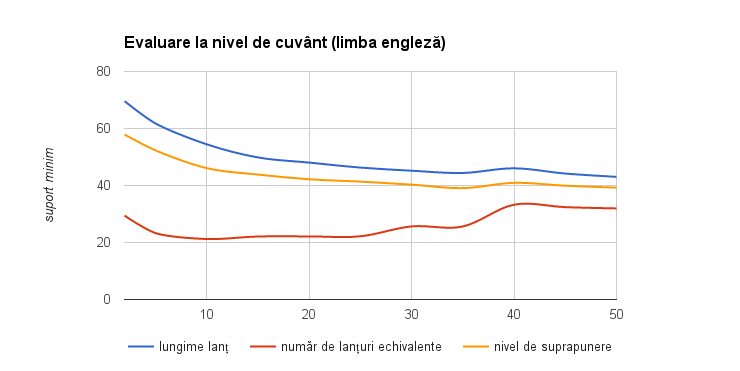
\includegraphics[width=1\textwidth]{figures/strategies-word-en.png}
    \caption{Evaluare comparativă a strategiilor pentru limba engleză($\%m_w$)}
    \label{fig:strategies-word-en}
\end{figure}

\begin{figure}[h!]
    \centering
    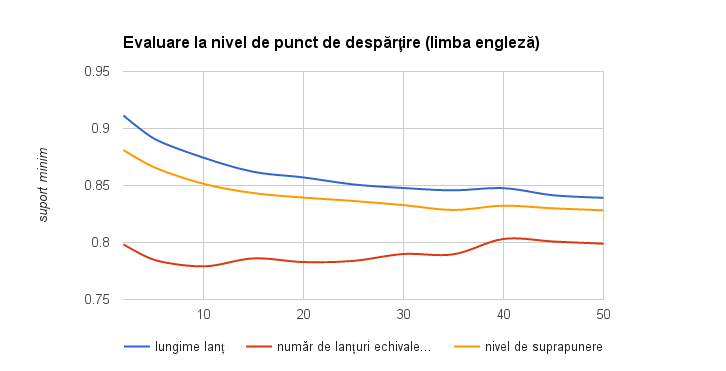
\includegraphics[width=1\textwidth]{figures/strategies-point-en.png}
    \caption{Evaluare comparativă a strategiilor pentru limba engleză($m_d$)}
    \label{fig:strategies-point-en}
\end{figure}


Din punct de vedere comparativ, în cadrul figurilor~\ref{fig:strategies-point-en} și~\ref{fig:strategies-word-en} se pot observa valorile prezentate în tabele anteriore.

După cum o arată și graficele, deși nu s-a obținut aceiași precizie ca și în cazul limbii române, fără vreo modificare a metodei pot fi realizate corect ~7 din 10 predicții corecte. 

\section{Evaluarea timpului de identificare de tipare frecvente}

Initial, înainte de a realiza predicții, este necesară identificarea tiparelor frecvente. Pentru a avea o imagine realistă asupra timpului de execuție necesar acestei etape, în cadrul tabelei~\ref{table:bide-en} sunt prezentate rezultele masurătorilor în cadrul setul de date conținând cuvinte silabisite în limba engleză.

Trebuie menționat că timpii raportați reprezintă: timpul de citire al datelor de pe disc, parsarea acestora și  identificarea tiparelor frecvente.

La nivelul~\ref{fig:bide-count-en} este ilustrată evoluția numărului de tipare identificate.

Iar în cadrul~\ref{fig:bide-runtime-en} se poate vedea evoluția timpului de execuție în funcție de suportul minim utilizat.

\begin{table}[h!]
\centering
\begin{tabular}{|c|c|c|}
\hline
suport minim & numar de tipare & timp de execuție (secunde)\\ 
\hline
50 & 3005 & 21.58\\ 
\hline
45 & 3426 & 22.33\\ 
\hline
40 & 3960 & 26.75\\ 
\hline
35 & 4683 & 26.83\\ 
\hline
30 & 5644 & 34.50\\ 
\hline
25 & 7114 & 38.34\\ 
\hline
20 & 9378 & 46.65\\ 
\hline
15 & 13141 & 58.57\\ 
\hline
10 & 21179 & 64.161\\ 
\hline
5 & 47795 & 113.63\\ 
\hline
2 & 135084 & 174.38125\\ 
\hline
\hline\end{tabular}
\label{table:bide-en}
\caption{Evaluarea timpului necesar identificări de tipare frecvente} 
\end{table}


La nivelul~\ref{fig:bide-count-en} este ilustrată evoluția numărului de tipare identificate.

Iar în cadrul~\ref{fig:bide-runtime-en} se poate vedea evoluția timpului de execuție în funcție de suportul minim utilizat.

\newpage
\begin{figure}[h!]
    \centering
    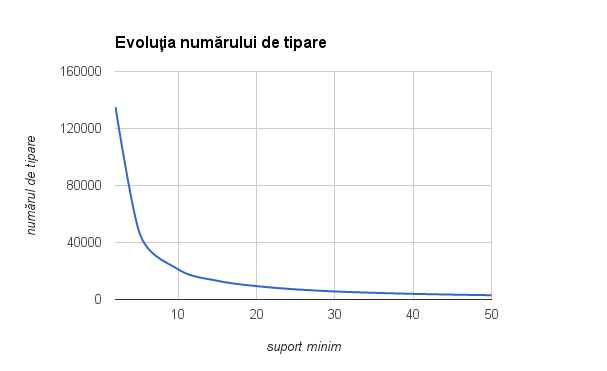
\includegraphics[width=.9\textwidth]{figures/bide-count-en.png}
    \caption{Evoluția numărului de tipare în funcție de suportul minim}
    \label{fig:bide-count-en}
\end{figure}

\begin{figure}[h!]
    \centering
    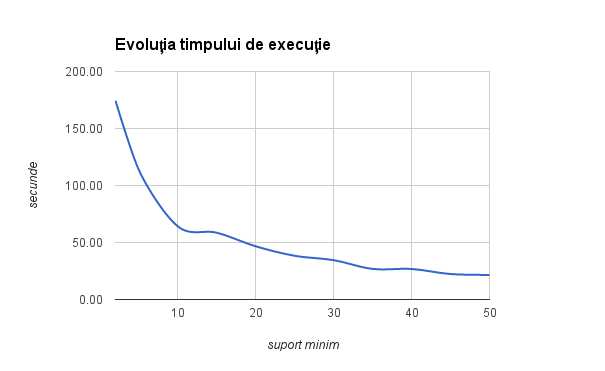
\includegraphics[width=.9\textwidth]{figures/bide-runtime-en.png}
    \caption{Evoluția timpul execuție pentru identificarea tiparelor frecvente}
    \label{fig:bide-runtime-en}
\end{figure}



\section{Evaluarea timpului de predicție}

Pentru a evalua timpul de execuție în cazul predicțiilor de silabificări au fost realizate o serie de masurători folosind setul de date descris în secțiunea precedentă: cuvinte în limba engleză (5000 de cuvinte de test, 182175 de cuvinte pentru identificarea tiparelor frecvente). 

La nivel de hardware s-a folosit o mașină dotată cu procesor Intel i5-3210M @ 2,5 GHz și 12 GB RAM.

Pentru fiecare strategie, în cadrul graficului~\ref{fig:runtime} este prezentat timpul mediu de silabisire (timpul total pentru predicția a 5000 de silabisiri / 5000)

\begin{figure}[h!]
    \centering
    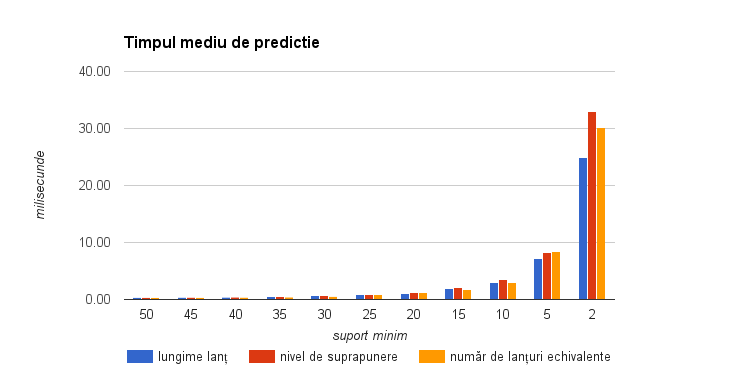
\includegraphics[width=1\textwidth]{figures/runtime.png}
    \caption{Timpul mediu de predicție în funcție de suportul minim utilizat și strategia de predicție}
    \label{fig:runtime}
\end{figure}

